\documentclass[titlepage]{article}
\usepackage{pdfpages}

\title{%
Bake By Weight\\
\large A Scientific Approach to Standardized Baking}

\author{Michael Gicking\\ Anybody who helps in a significant manner}

\begin{document}
\maketitle
Table of Contents
\begin{enumerate}
	\item Introduction
	\item Thanks
	\item Cookies
	\item Pastries
	\item Breakfast
	\item Breads
	\item Biscuits
		\begin{itemize}
			\item American Biscuits
			\item Scones
		\end{itemize}
	\item Pasta
	\item Glossary
\end{enumerate}

\pagebreak
\section*{Introduction}
This book started out as a conversation with some coworkers of the danger of cooking with measuring cups. That being, not all powdered solids are made equal. For example, a single cup of flour can range anywhere from 4 to 6 ounces due to things like age, humidity, or even whether you scooped from the top of the bag or the bottom. As a result, this book aims to provide a collection of recipes, common and not-so-common alike, that use weight as the primary measuring methodology in order to standardize your baking. That's not to say that ALL ingredients will be listed solely by mass. Water, for example, does a wonderful job of not compressing, so a liter is a liter is a liter. That said, even in cases where mass isn't necessary, we will still provide it for you, just to make things easier.
\vspace{\baselineskip}

\noindent Our recommendation for you while reading this book is to invest in a stand mixer and a good digital scale with a tare button. It is absolutely a game changer to have both these tools since it will make baking easier, quicker, and eliminates the hard math and back-breaking kneading (for the most part). In short, it will make baking fun, or at least more fun than it already is!
\vspace{\baselineskip}

\noindent We hope you will enjoy this cookbook and will consider sharing its recipes and insights with your loved ones much the same as we do with ours.
\section*{Thanks}
Thanks to my friends and coworkers who've shared recipes they love with me in the hopes of getting them converted. Without your recipes, this book never could have been done.
\vspace{\baselineskip}

\noindent Special thanks to those who have helped me pull off these conversions by testing my recipes.
\vspace{\baselineskip}

\noindent Finally, thank you to friends, family, and God for providing me with the emotional support to pull this endeavor off.
\pagebreak
\section{Cookies}
Cookies are the first step in our culinary journey of baking for a couple of reasons. The primary reason being because who doesn't like cookies? Another great quality of cookies is that they are usually quite forgiving, and give you much more than normal leeway when it comes to baking to experiment. As such, you'll notice that not all measurements in the recipes contained in the chapter are weight-based. This is because the precision of these ingredients doesn't matter as much. For example, you could choose to include more chocolate chips in our Classical Chocolate Chip recipe, or you could do less. Consider substituting a portion of the chocolate chips with crushed or chopped nuts. It's entirely up to you and the possibilities are endless.
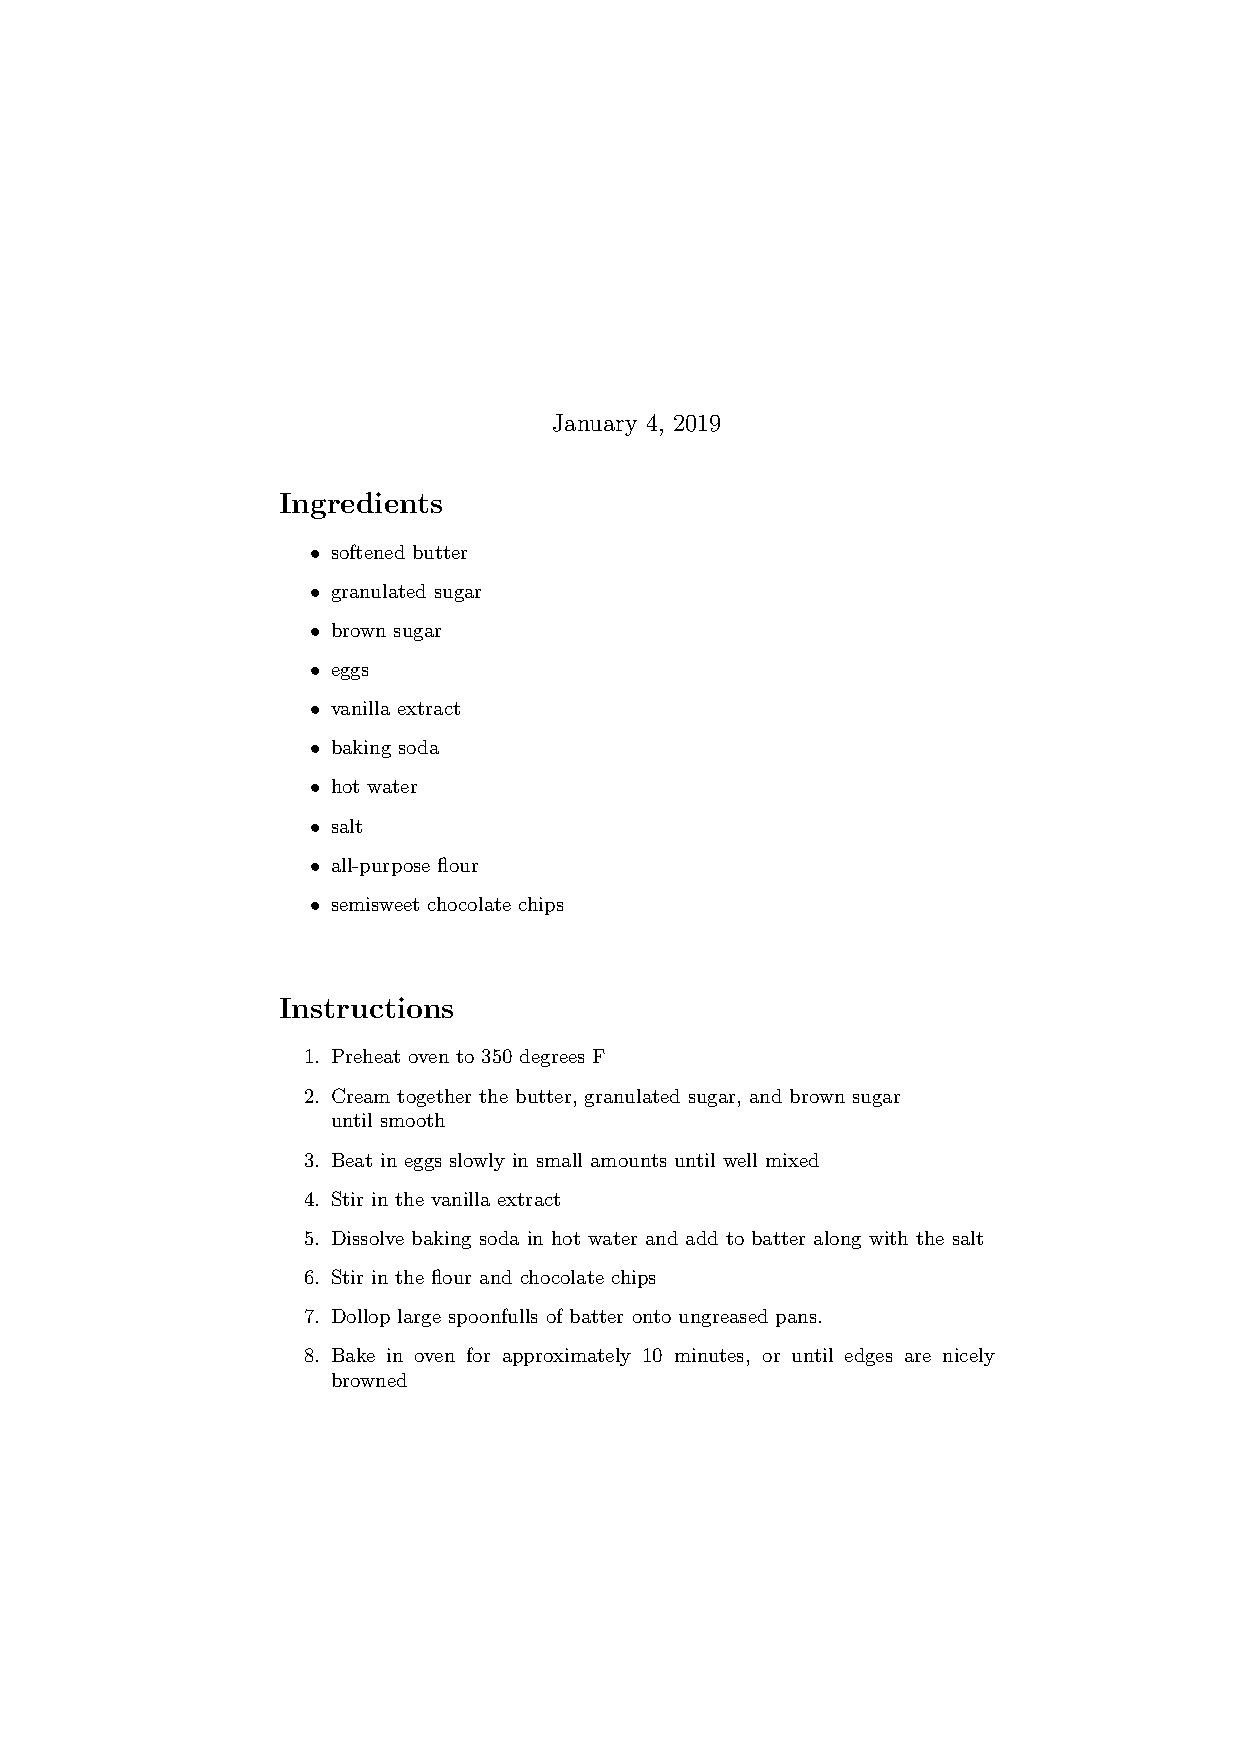
\includepdf[pagecommand=\subsection{Classical Chocolate Chip}]{chocolateChipCookies}
\pagebreak
\section{Pastries}
\pagebreak
\section{Breakfast}
\pagebreak
\section{Breads}
\pagebreak
\section{Biscuits}
\pagebreak
\section*{Glossary}
\end{document}